\documentclass[12pt]{article} 

%\usepackage[T1]{fontenc}
%\usepackage{lmodern}
%\usepackage[urw-garamond]{mathdesign}

%\usepackage{times,helvet}

%\usepackage{fourier}
%\usepackage{fourier}
%\usepackage[scaled=0.85]{berasans}
%\usepackage[scaled=0.85]{beramono}

%Palatino+Mathpazo
%==============

\usepackage[T1]{fontenc}
\usepackage{palatino}
\usepackage[scaled=0.90]{helvet}
\usepackage{mathpazo}
\usepackage{textcomp}

%Fourier
%==============

%\usepackage[T1]{fontenc}
%\usepackage[scaled=0.90]{helvet}
%\usepackage{fourier}
%\usepackage{textcomp}

%Palatino+Euler
%===============

%\usepackage[T1]{fontenc}
%\usepackage{palatino}
%\usepackage[scaled=0.90]{helvet}
%\usepackage{eulervm}
%\usepackage{textcomp}

%Mathdesign (Utopia)
%===============

%\usepackage[T1]{fontenc}
%\usepackage[scaled=0.90]{helvet}
%\usepackage[utopia]{mathdesign}%%{fourier}
%\usepackage{textcomp}

%\usepackage{ssss}
\usepackage{amsmath}
\usepackage{amsbsy}
%\usepackage(amssymb}
\usepackage{fancyhdr}
\usepackage{tabularx}
\usepackage{verbatim,alltt}
\usepackage{moreverb}
\usepackage{float}
%\usepackage{deflist}
\usepackage{graphicx}
\usepackage{longtable}
\usepackage{portland}
\usepackage{sectsty}
\usepackage{longtable}
\usepackage{color}
\usepackage{fancyvrb}
\usepackage{booktabs}

%must be last package
%\usepackage{hyperref}
\usepackage[debug=false, colorlinks=true, pdfstartview=FitV, linkcolor=blue, citecolor=blue, urlcolor=blue, pdfpagelabels=true]{hyperref}

%\usepackage{movie15}
\usepackage{media9}

\textwidth 6.5in
\textheight 9.5in
%\topmargin -.1in
\topmargin -.75in
\newlength{\boxwidth}
\setlength{\boxwidth}{5.8in}
\oddsidemargin -0in
\evensidemargin -0in
\headheight 0.25in
\lhead{{\sl 1D Hanford SX-115 Tank Leak}}
\chead{}
\rhead{\today}
\cfoot{\rm -- \thepage\ --}
\newcommand\flotran{{\sl PFloTran}}
\renewcommand{\baselinestretch}{1.5}
\def\EQ#1\EN{\begin{equation}#1\end{equation}}
\def\BA#1\EA{\begin{align}#1\end{align}}
\def\BS#1\ES{\begin{split}#1\end{split}}
%\newcommand{\EQ}{\begin{equation}}
%\newcommand{\EN}{\end{equation}}
\newcommand{\bc}{\begin{center}}
\newcommand{\ec}{\end{center}}
\newcommand{\eq}{\ =\ }
\newcommand{\degc}{$^\circ$C}
\newcommand{\ecm}{{\rm ecm}}
\newcommand{\eff}{{\rm eff}}
\newcommand{\eqr}{{\rm le}}
\newcommand{\equ}{{\rm eq}}
\newcommand{\kin}{{\rm kin}}
\newcommand{\rdx}{{\rm rdx}}
\newcommand{\ind}{{\rm id}}
\newcommand{\dep}{{\rm dp}}
\newcommand{\e}{{\rm{e}}}
\newcommand{\erf}{{\rm{erf}}}
\newcommand{\erfc}{{\rm{erfc}}}
\newcommand{\p}{{\partial}}
\newcommand{\A}{{\mathcal A}}
\newcommand{\B}{{\mathcal B}}
\newcommand{\C}{{\mathcal C}}
\newcommand{\AC}{{\mathcal AC}}
\newcommand{\BC}{{\mathcal BC}}
\newcommand{\D}{{\mathcal D}}
\newcommand{\E}{{\mathcal E}}
\newcommand{\F}{{\mathcal F}}
\newcommand{\G}{{\mathcal G}}
\newcommand{\J}{{\mathcal J}}
\newcommand{\K}{{\mathcal K}}
\newcommand{\M}{{\mathcal M}}
\newcommand{\N}{{\mathcal N}}
\newcommand{\cO}{{\mathcal O}}
\renewcommand{\P}{{{\mathcal P}}}
\newcommand{\Q}{{\mathcal Q}}
\newcommand{\R}{{{\mathcal R}}}
\renewcommand{\S}{{\mathcal S}}
\newcommand{\T}{{\mathcal T}}
\newcommand{\W}{{\mathcal W}}
\newcommand{\Y}{{\mathcal Y}}
\newcommand{\y}{{\mathcal y}}
\newcommand{\Z}{{\mathcal Z}}
\newcommand{\rev}{{\rm rev}}
\newcommand{\irr}{{\rm irr}}
\renewcommand{\a}{{\alpha}}
\newcommand{\abar}{{\bar\alpha}}
\renewcommand{\b}{{\beta}}
\newcommand{\s}{{\sigma}}
\renewcommand{\c}{{\rm CO_2}}
\newcommand{\w}{{\rm H_2O}}
\newcommand{\air}{{\rm N_2}}
\newcommand{\pe}{{\rm Pe}}
\newcommand{\da}{{\rm Da}}
\renewcommand{\k}{{\kappa}}
\renewcommand{\L}{\widehat{\mathcal L}}
\renewcommand{\bar}{\overline}
\newcommand{\dsty}{{\displaystyle}}
\newcommand{\diff}{{\mathcal D}}
\newcommand{\surf}{\equiv \!\!\!}
\newcommand{\bnabla}{\boldsymbol{\nabla}}
\newcommand{\bA}{\boldsymbol{A}}
\newcommand{\ba}{\boldsymbol{a}}
\newcommand{\bB}{\boldsymbol{B}}
\newcommand{\bC}{\boldsymbol{C}}
\newcommand{\bE}{\boldsymbol{E}}
\newcommand{\bF}{\boldsymbol{F}}
\newcommand{\bi}{\boldsymbol{i}}
\newcommand{\bI}{\boldsymbol{I}}
\newcommand{\bJ}{\boldsymbol{J}}
\newcommand{\bK}{\boldsymbol{K}}
\newcommand{\bM}{\boldsymbol{M}}
\newcommand{\bGamma}{\boldsymbol{\Gamma}}
\newcommand{\bOmega}{\boldsymbol{\Omega}}
\newcommand{\bPsi}{\boldsymbol{\Psi}}
\newcommand{\bO}{\boldsymbol{O}}
\newcommand{\bnu}{\boldsymbol{\nu}}
\newcommand{\bdS}{\boldsymbol{dS}}
\newcommand{\bq}{\boldsymbol{q}}
\newcommand{\br}{\boldsymbol{r}}
\newcommand{\bR}{\boldsymbol{R}}
\newcommand{\bS}{\boldsymbol{S}}
\newcommand{\bu}{\boldsymbol{u}}
\newcommand{\bv}{\boldsymbol{v}}
\newcommand{\bz}{\boldsymbol{z}}
\newcommand{\arrows}{~\rightleftharpoons~}
\newcommand{\arrowstab}{\!\!\!\rightleftharpoons\!\!\!}
\newcommand{\longline}{\noindent\rule[-0.1in]{\textwidth}{0.01in}}

%\numberwithin{equation}{section}
%\renewcommand{\theequation}{\arabic{section}.\arabic{equation}}

\setcounter{secnumdepth}{5}
\setcounter{tocdepth}{5}
\setcounter{equation}{0}
\setcounter{section}{1}

%\setlength{\parindent}{0.3125in}
%\setlength{\parskip}{2ex plus 0.2ex minus 0.2ex}

\renewcommand{\contentsname}{TABLE OF CONTENTS}
\setcounter{secnumdepth}{5}

\setlongtables

\sectionfont{\nohang\centering} 

\pagestyle{fancy}

\thispagestyle{empty}

%\renewcommand{\thepage}{\roman{page}}
\renewcommand{\thepage}{\arabic{page}}

\allowdisplaybreaks[1]

\begin{document}

\section*{Problem Description of Modeling a Leak from the SX-115 Tank at the Hanford S/SX Tank Farm}

 P.C. Lichtner 
 
\noindent \today

\section*{Problem Description}

The saturation profile is computed for both steady-state and transient conditions in a 1D vertical column consisting of a layered porous medium representing the Hanford sediment in the vicinity of the S/SX tank farm. The transient case simulates a leak from the base of the SX-115 tank. This problem description is taken from Lichtner et al. (2004).

\section*{Governing Equations}

The moisture profile is calculated using parameters related to the Hanford sediment at the S/SX tank farm based on the Richards equation for variably saturated porous media. The Hanford sediment is composed of five layers with the properties listed in Tables~\ref{t1} and \ref{t2}. The governing equations consist of Richards equation for variably saturated fluid flow given by
\EQ
\frac{\p}{\p t} \varphi s\rho + \bnabla\cdot\bq\rho \eq Q,
\EN
and solute transport of a tracer
\EQ
\frac{\p}{\p t}\varphi C + \bnabla\cdot\big(\bq C - \varphi s \tau D \bnabla C\big) \eq Q_C.
\EN
In these equations $\varphi$ denotes the spatially variable porosity of the porous medium assumed to constant within each stratigraphic layer, $s$ gives the saturation state of the porous medium, $\rho$ represents the fluid density in general a function of pressure and temperature, $C$ denotes the solute concentration, $D$ denotes the diffusion/dispersion coefficient, $\tau$ represents tortuosity, $Q$ and $Q_C$ denote source/sink terms, and $\bq$ denotes the Darcy velocity defined by
\EQ
\bq\eq - \frac{k_{\rm sat}k_r}{\mu} \bnabla (p-\rho g z),
\EN
with saturated permeability $k_{\rm sat}$, relative permeability $k_r$, fluid viscosity $\mu$, pressure $p$, formula weight of water $W$, acceleration of gravity $g$, and height $z$. Van Genuchten capillary properties are used for relative relative permeability according to the relation
\EQ\label{kr}
k_{r} \eq \sqrt{s_{\rm eff}} \left\{1 - \left[ \left( s_l^{\rm 
eff} \right)^{1/m} \right]^m \right\}^2, 
\EN
where $s_{\rm eff}$ is related to capillary pressure $P_c$ by the equation
\EQ\label{sat}
s_{\rm eff} \eq \left[1+\left( \alpha |P_c| \right)^n 
\right]^{-m}, 
\EN 
where $s_{\rm 
eff}$ is defined by 
\EQ\label{seff}
s_{\rm eff} \eq \frac{s - s_r}{1 - s_r}, 
\EN 
and where $s_r$ denotes the residual saturation. The quantity $n$ is related to $m$ by the expression 
\EQ\label{lambda} 
m \eq 1-\frac{1}{n}, \ \ \ \ \ n \eq \frac{1}{1-m}. 
\EN 
The capillary pressure $P_c$ and fluid pressure $p$ are related by the (constant) gas pressure $p_g^0$
\EQ
P_c \eq p_g^0-p,
\EN
where $p_g^0 \!=\! 101,325$ Pa is set to atmospheric pressure.

\section*{Semi-Analytical Solution for Steady-State Conditions}

For steady-state conditions the saturation profile satisfies the equation
\EQ
\frac{d}{dz} \rho q_z \eq 0,
\EN
or assuming an incompressible fluid
\EQ
q_z \eq q_z^0,
\EN
where $q_z^0$ denotes infiltration at the surface. Thus the pressure is obtained as a function of $z$ by solving the ODE
\EQ
\frac{dp}{dz} \eq -\frac{\mu q_z^0}{k_{\rm sat} k_r} - \rho g,
\EN
using Eqns.\eqref{kr} and \eqref{sat} to express the relative permeability $k_r$ as a function of pressure. For the special case of zero infiltration it follows that
\EQ
p(z) \eq p_0 - \rho g (z-z_0),
\EN
with $p(z_0)\!=\!p_0$. The saturation profile is obtained from Eqns.\eqref{sat} and \eqref{seff}.

\section*{Model Parameters}

Model parameters used in the simulations are listed in Tables~\ref{t1} and \ref{t2}. Although not needed here, thermal properties are also listed. Diffusivity was set to $10^{-9}$ m$^2$ s$^{-1}$ and tortuosity was set to one.

\renewcommand{\tabcolsep}{1.7mm}

\begin{table}[H]\centering
\caption{Stratigraphic sequence used in the calculations, after Ward et al. (1996).}\label{t1}

\vspace{3mm}

\begin{tabular}{lcr}
\toprule
Formation & Abbrev. & Thickness [m]\\
\midrule
Backfill & BF & 16.0\\
Hanford Fine Sand & HF & 23.0\\
Plio-Pleistocene & PP & 6.0\\
Upper Ringold Gravel & URG & 3.0\\
Middle Ringold Gravel & MRG & 20.0\\
\bottomrule
\end{tabular}
\end{table}

\begin{table}[H]\centering
\caption{Parameters for material and thermal properties for intrinsic rock density $\rho_s$, heat capacity $c$, thermal conductivity $\kappa$, porosity $\varphi$, residual water saturation $s_r$, van Genuchten parameters $\alpha$ and $\lambda$, and vertical water saturated permeability $k_{\rm sat}$. Data taken from Khaleel and Freeman (1995), Khaleel et al. (2001), and Pruess et al. (2002).}\label{t2}

\vspace{3mm}

\begin{tabular}{lccccccccc}
\toprule
Formation & $\rho_s$ & $c$ & $\kappa_{\rm dry}$ & $\kappa_{\rm wet}$ & $\varphi$ & $s_r$ & $\alpha$ & $m$ & $k_{\rm sat}$\\
& g cm$^{-3}$ & J kg$^{-1}$ K$^{-1}$ & \multicolumn{2}{c}{W m$^{-1}$} & --- & --- & m$^{-1}$ & --- & m$^2$\\
\midrule
BF  & 2.8 & 800 & 0.5 & 2 & 0.2585 & 0.0774 & 1.008e-3 & 0.658  &1.24e-12\\
HF  & 2.8 & 800 & 0.5 & 2 & 0.3586 & 0.0837 & 9.390e-5 & 0.469  &1.23e-13\\
PP  & 2.8 & 800 & 0.5 & 2 & 0.4223 & 0.2595 & 6.840e-5 & 0.456  &1.37e-14\\
URG & 2.8 & 800 & 0.5 & 2 & 0.2625 & 0.2130 & 2.961e-5 & 0.386  &5.27e-14\\
MRG & 2.8 & 800 & 0.5 & 2 & 0.1643 & 0.0609 & 6.330e-5 & 0.392  &7.33e-14\\
\bottomrule
\end{tabular}
\end{table}

\section*{Simulation Results}

The calculations are carried out for an isothermal system using Richards equation. First, the steady-state saturation profile is obtained without the tank leak present. Then using the steady-state profile as the initial condition the tank leak is turned on. The results for the steady-state saturation and pressure profiles are shown in Figure~\ref{f1} for infiltration rates at the surface of 0, 8 and 80 mm/y. The mean infiltration rate at the Hanford site is approximately 8 mm/y. A 1D column 68 m heigh with the water table located at a height of 6 m from the bottom is used in the simulation. A uniform grid spacing of 0.5 m is used to discretize Richards equation.

Shown in Figure~\ref{f2} is the saturation at different times following a two week leak releasing 60,000 gallons from the SX-115 tank at a depth of 16 m. In the simulation a release rate of $1.87\!\times\! 10^{-3}$ kg/s is used.

%\clearpage

\section*{References}

\begin{description}

\item Khaleel, R., E.J. Freeman (1995) Variability and scaling of hydraulic properties for 200 area soils, Hanford Site. Report WHC-EP-0883. Westinghouse Hanford Company, Richland, WA.

\item Khaleel, R., T.E. Jones, A.J. Knepp, F.M. Mann, D.A. Myers, P.M. Rogers, R.J. Serne, and M.I. Wood (2000) Modeling data package for S-SX Field Investigation Report (FIR). Report RPP-6296, Rev. 0. CH2M Hill Hanford Group, Richland, WA.

\item Lichtner, P.C., Yabusaki, S.B., Pruess K., and Steefel, C.I. (2004) Role of Competitive Cation Exchange on Chromatographic Displacement of Cesium in the Vadose Zone Beneath the Hanford S/SX Tank Farm, {\em VJZ}, {\bf 3}, 203--219.

\item Pruess, K., S. Yabusaki, C. Steefel, and P. Lichtner (2002) Fluid flow,
heat transfer, and solute transport at nuclear waste storage tanks in the Hanford vadose zone. Available at www.vadosezonejournal.org. Vadose Zone J. 1:68--88.

\end{description}

\clearpage

\begin{figure}[h]\centering
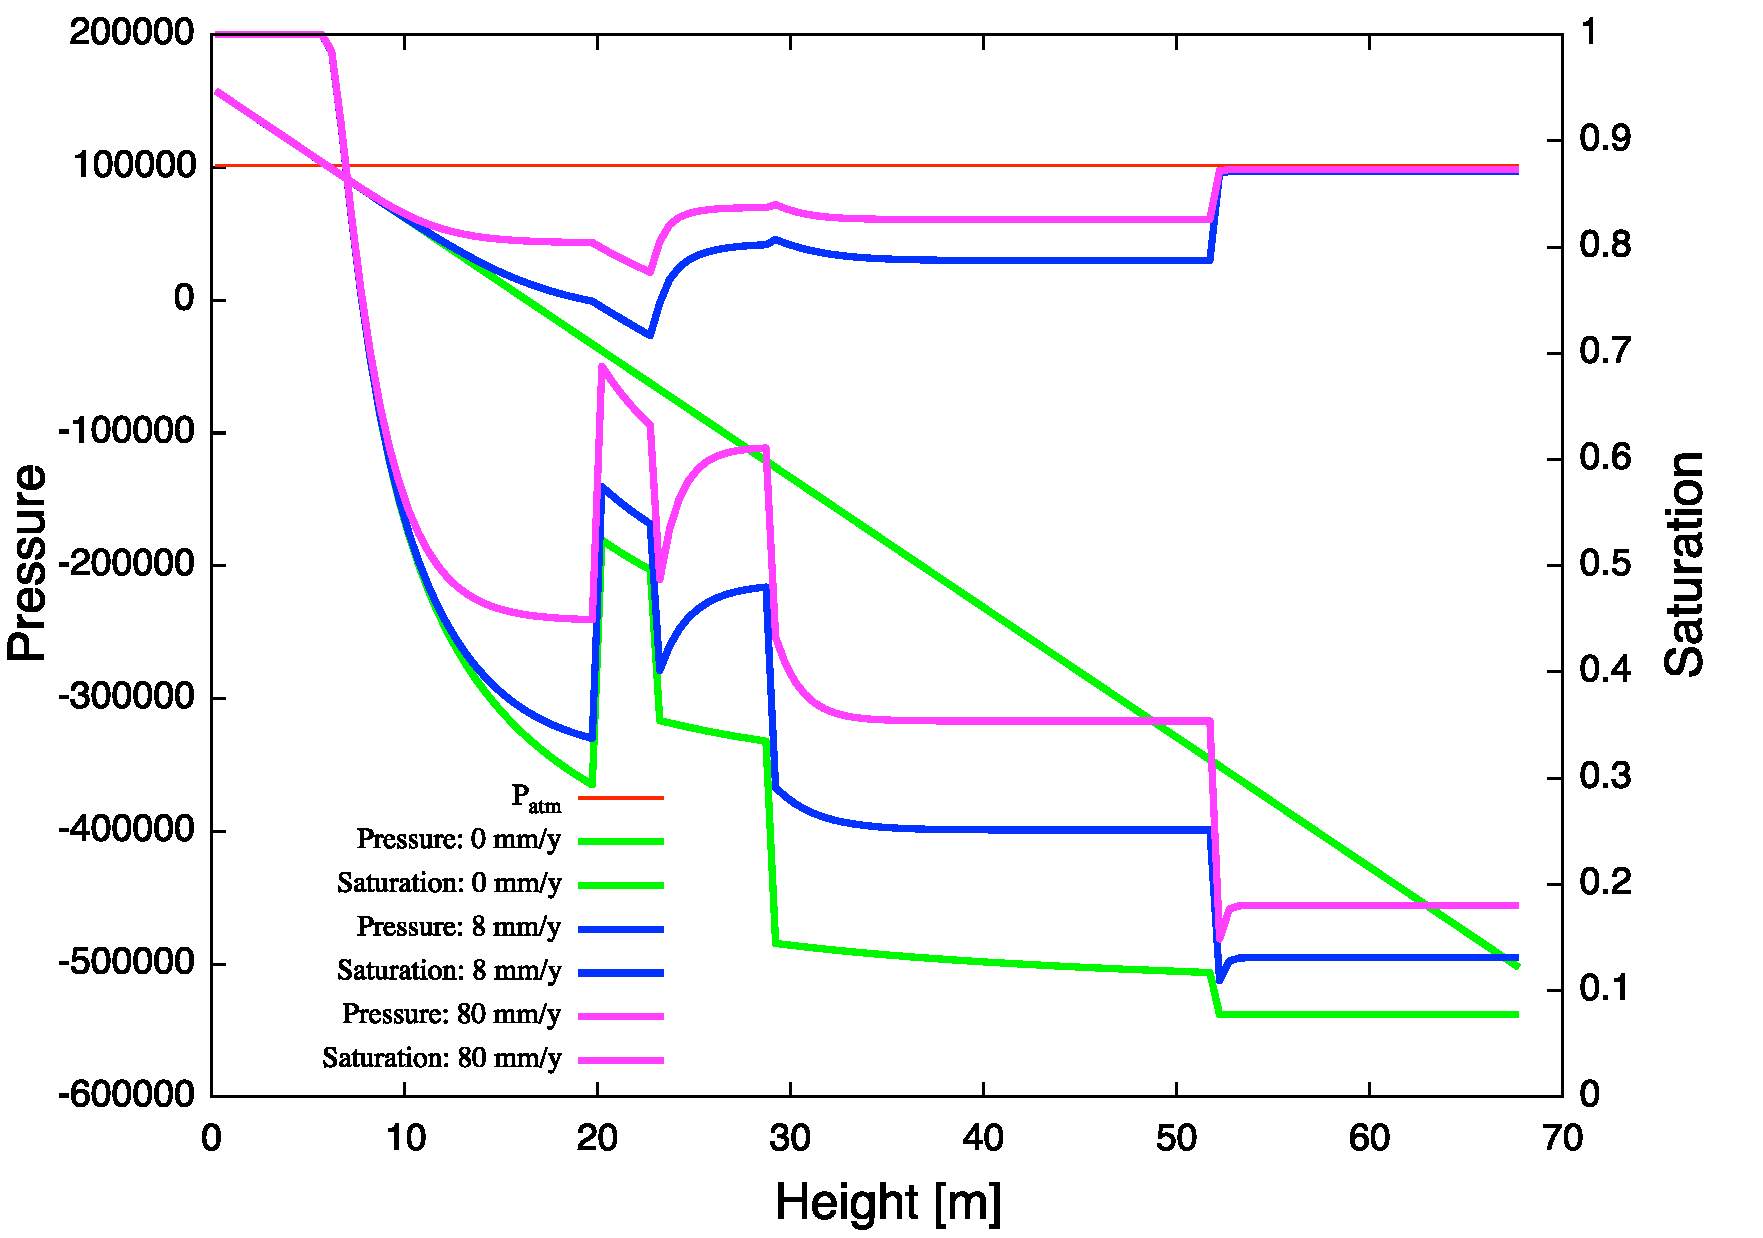
\includegraphics[scale=0.45]{./figs/ps}
\caption{Steady-state saturation and pressure profiles for infiltration rates of 0, 8 and 80 mm/y. The water table is located at 6 m from the bottom of the computational domain.}\label{f1}
\end{figure}

\begin{figure}[h]\centering
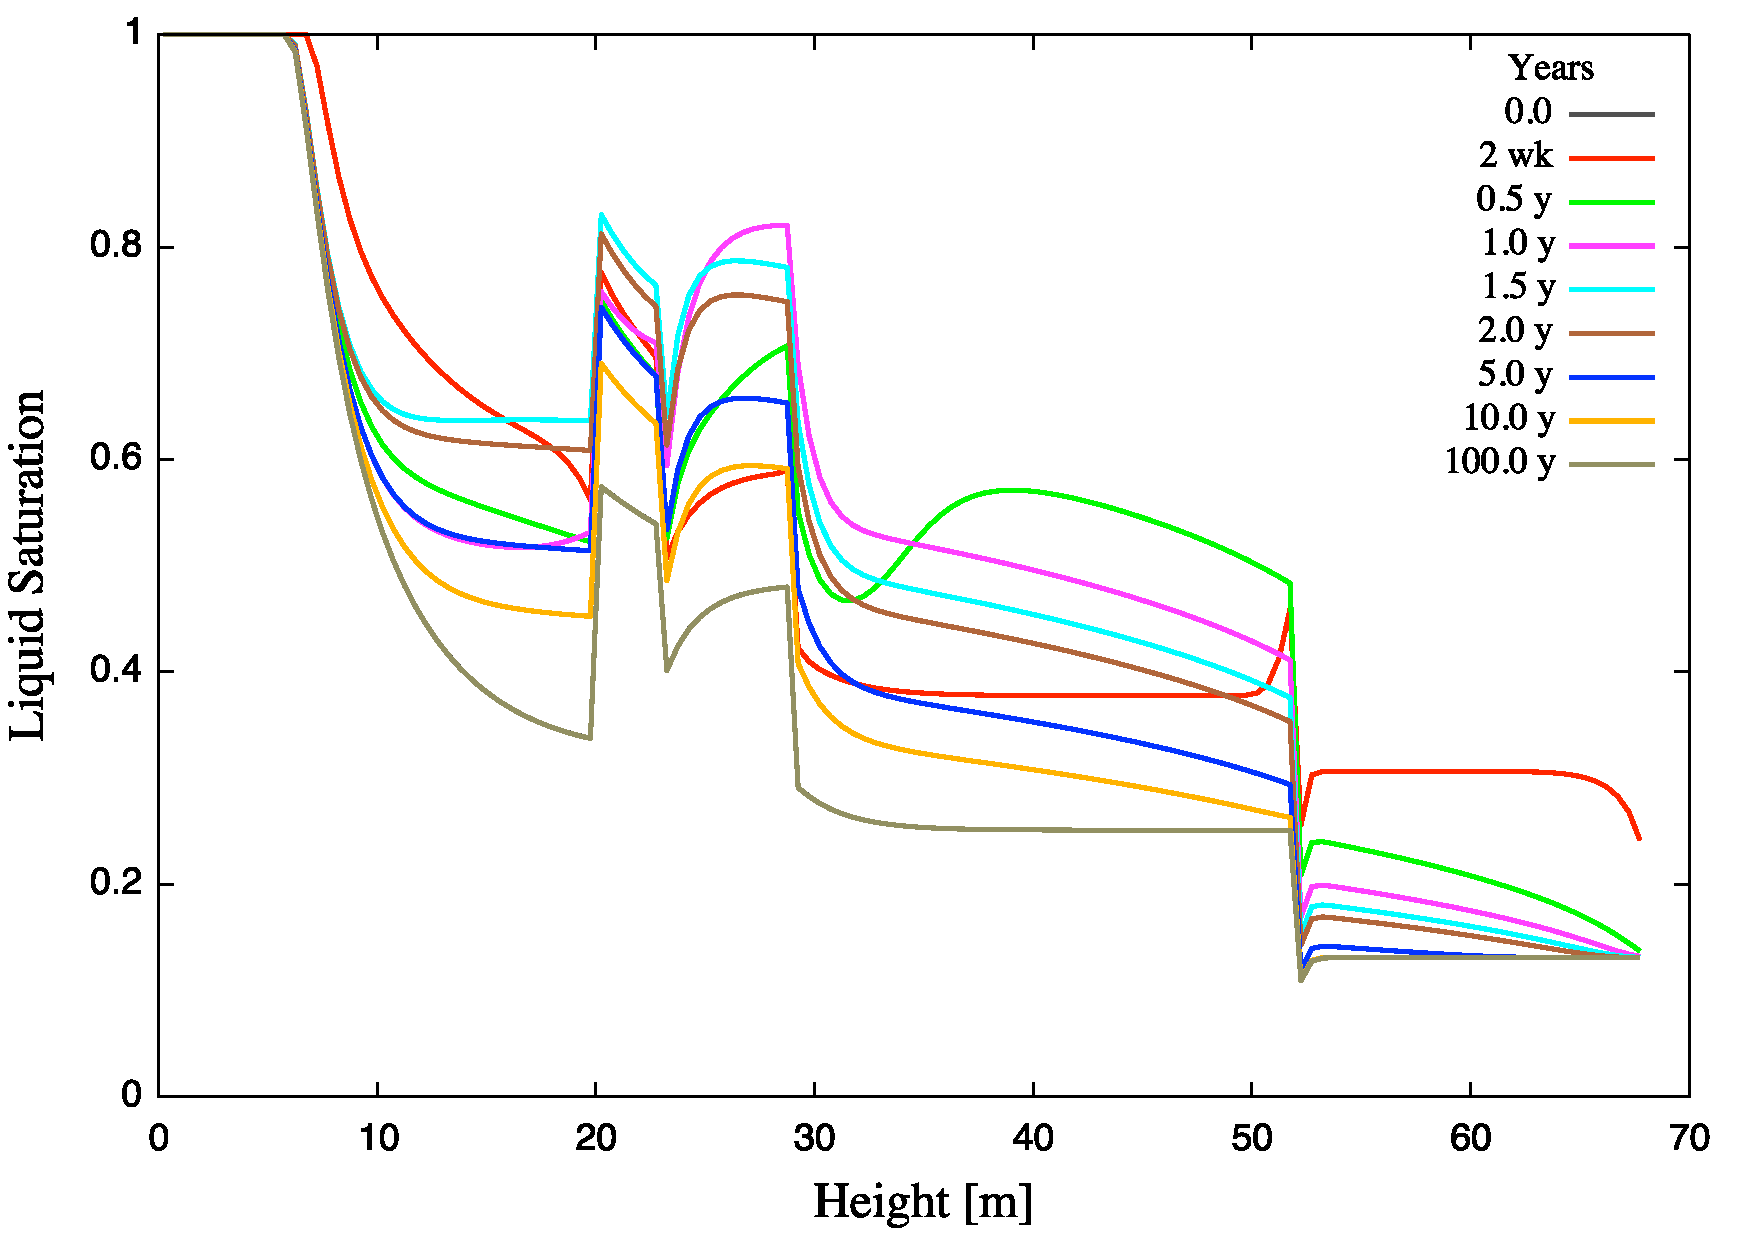
\includegraphics[scale=0.45]{./figs/sat_leak}
\caption{Simulation of a tank leak with a duration of two weeks showing the saturation profile for different times indicated in the figure.}\label{f2}
\end{figure}

\begin{figure}[h]\centering
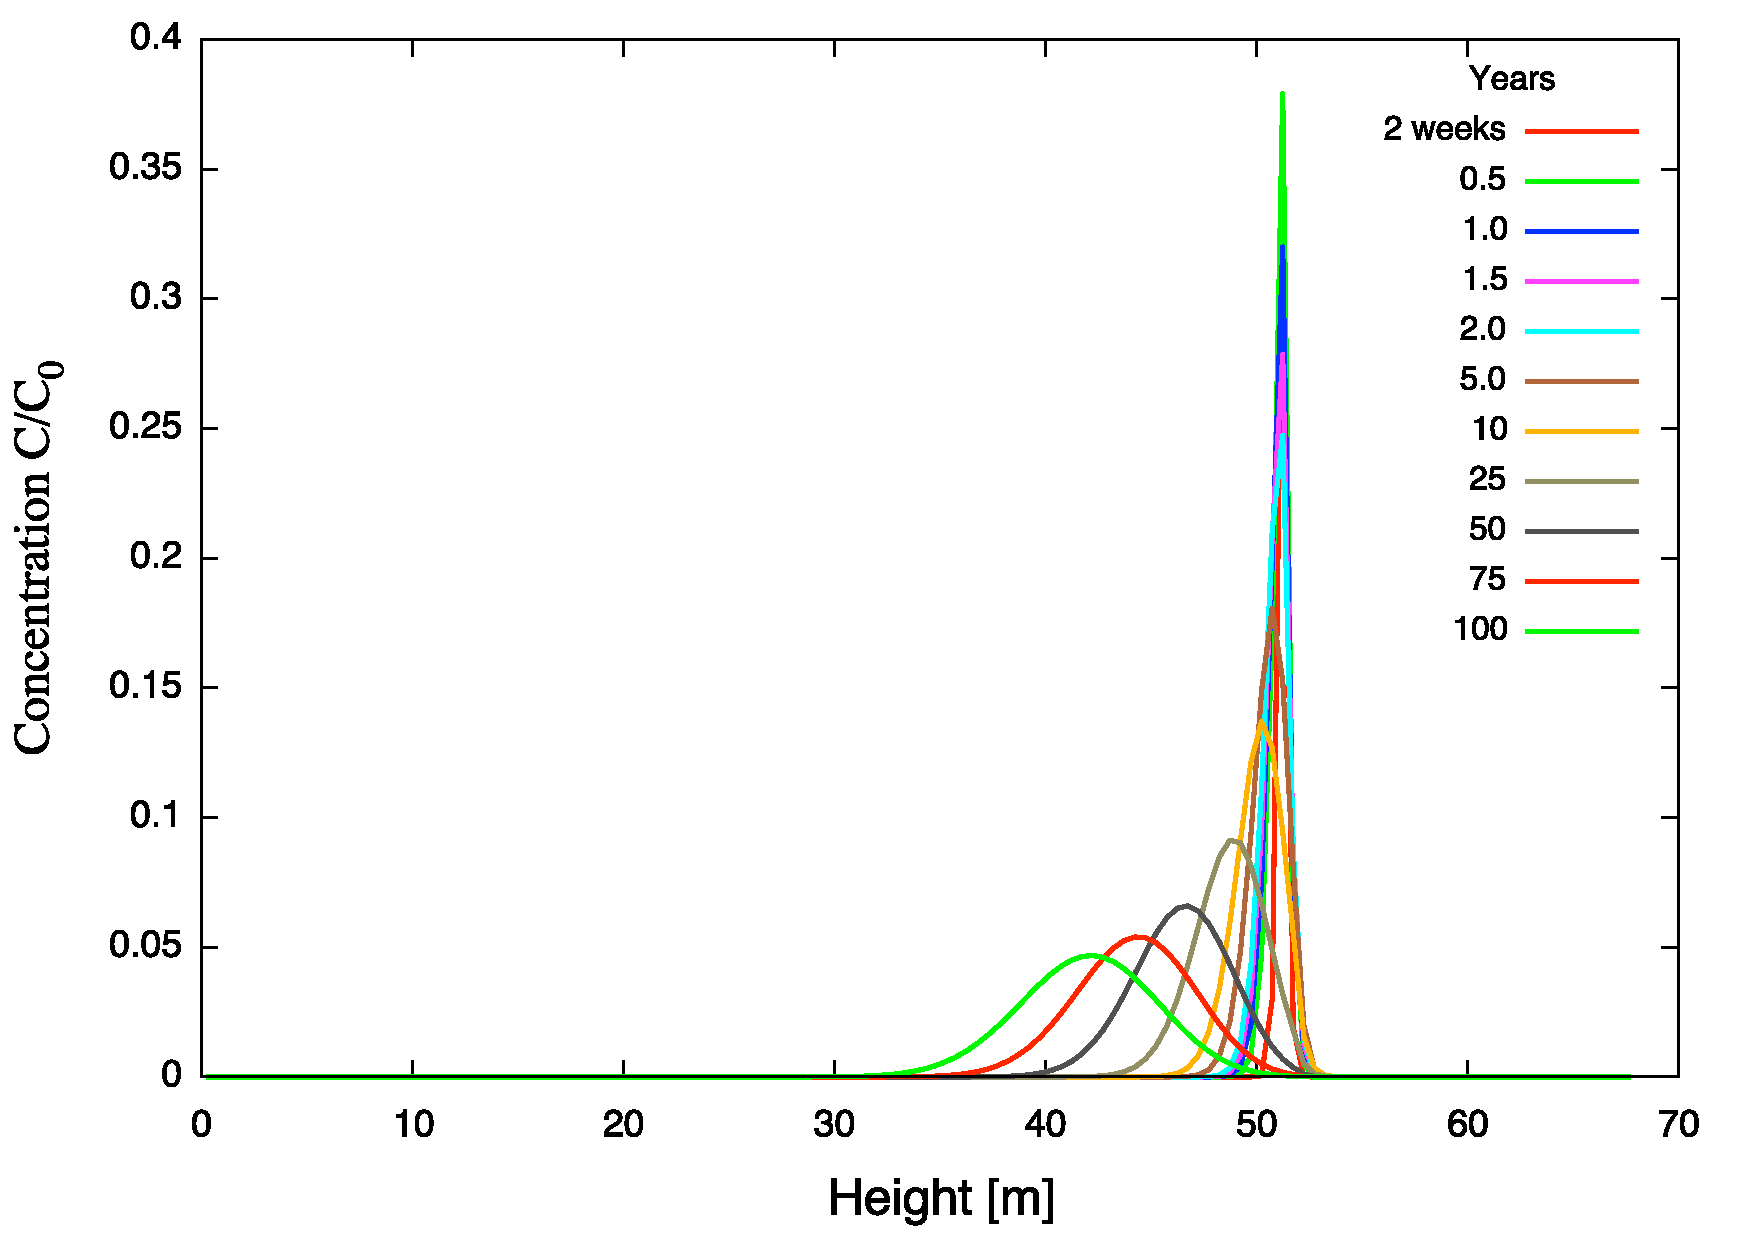
\includegraphics[scale=0.45]{./figs/conc}
\caption{The solute concentration profile corresponding to Figure~\ref{t2} for different times indicated in the figure.}\label{f3}
\end{figure}

\clearpage

\section*{PFLOTRAN Input Files}

Listing of PFLOTRAN input file including a tracer. Note that the stratigraphic zone specification in {\tt REGION} is grid independent as is the grid size specification in keyword {\tt GRID}. Therefore to change the grid spacing only the line: {\tt NXYZ 1 1 136}, needs to be changed. Also note that a line beginning with a colon (:) is read as a comment.

\bigskip

\noindent PFLOTRAN input file {\tt pflotran.in}: 
\tiny
%\footnotesize
\verbatiminput{pflotran.in}

\clearpage

\normalsize
\noindent
Source/sink file {\tt src.dat}:
\footnotesize
\verbatiminput{src.dat}

\end{document}
